\chapter{Цифровая модуляция}
\section{Постановка задачи}
\begin{enumerate}
\item 
Получить сигналы BPSK, PSK, OQPSK, genQAM, MSK, M-FSK модуляторов.
\item
Построить их сигналы
\item
Провестисравнение изученных методов модуляции цифровых сигналов.
\end{enumerate}
\section{Теоретическая часть}
Сущность цифровой модуляции заключается в том, что передаваемый непрерывный сигнал дискретизируется во времени, квантуется по уровню и полученные отcчеты, следующие в дискретные моменты времени, преобразуются в кодовые комбинации. Полученной последовательностью кодовых видеосигналов модулируется высокочастотный сигнал-переносчик.
Существует 3 основных вида манипуляции сигналов: амплитудная (Amplitude-shift keying (ASK)), частотная (Frequency-shift keying (FSK)) и фазовая (Phase-shift keying (PSK)).
\begin{enumerate}
\item Амплитудная манипуляция (ASK) — изменение сигнала, при котором скачкообразно меняется амплитуда несущего колебания. 
\item При частотной манипуляции (FSK) значениям «0» и «1» информационной последовательности соответствуют определённые частоты синусоидального сигнала при неизменной амплитуде. Частотная манипуляция весьма помехоустойчива. Однако при частотной манипуляции неэкономно расходуется ресурс полосы частот телефонного канала. Поэтому этот вид модуляции применяется в низкоскоростных протоколах, позволяющих осуществлять связь по каналам с низким отношением сигнал/шум.
\item Фазовая манипуляция (PSK) — один из видов фазовой модуляции, при которой фаза несущего колебания меняется скачкообразно в зависимости от информационного сообщения.
\end{enumerate}
Этот набор манипуляций определяется основными характеристиками, которыми обладает любой сигнал. Для моделирования модуляции цифрового сигнала в ходе лаботаторной работы предлагается использовать следующий набор функций:
\begin{enumerate}
\item Функция randerr предназначена для формирования ошибок в цифровом сигнале. Она дает матрицу, в каждой строке которой имеется заданное число случайно расположенных ненулевых элементов.
\item Для оценки помехоустойчивости системы связи необходимо произвести сравнение исходного (передаваемого) сообщения с сообщением, полученным в результате приема, и определить число ошибок, возникших в процессе передачи, а также вероятность ошибки. Эти действия выполняются функциями symerr и biterr, первая из которых подсчитывает число несовпадающих символах в двух сообщениях, а вторая — число несовпадающих битов в двоичных представлениях этих символов. Кроме числа ошибок, обе функции могут возвращать долю ошибок в общем числе символов (битов) и индикаторы мест возникновения ошибок.
\item Последние две функции данной группы предназначены для графического отображения сигналов с квадратурной манипуляцией. Функция eyediagram выводит так называемую глазковую диаграмму, а функция scatterplot — диаграмму рассеяния.
\end{enumerate}

\section{Ход работы}

\subsection{Код matlab}
\begin{lstlisting}
%BPSK modulation
h = modem.pskmod('M', 2);
g = modem.pskdemod('M', 2);
msg = randint(10,1,2);
modSignal = modulate(h,msg);
errSignal = (randerr(1,10, 3) ./ 30)';
modSignal = modSignal + errSignal;
demodSignal = demodulate(g,modSignal);
scatterplot(modSignal);
eyediagram(modSignal,10);
scatterplot(demodSignal);
eyediagram(demodSignal,10);

%PSK modulation
h = modem.pskmod('M', 8);
g = modem.pskdemod('M', 8);
msg = randint(10,1,8);
modSignal = modulate(h,msg);
errSignal = (randerr(1,10, 3) ./ 30)';
modSignal = modSignal + errSignal;
demodSignal = demodulate(g,modSignal);
scatterplot(modSignal);
eyediagram(modSignal,10);
scatterplot(demodSignal);
eyediagram(demodSignal,10);

%OQPSK modulation
h = modem.oqpskmod;
g = modem.oqpskdemod;
msg = randint(200,1,4);
modSignal = modulate(h,msg);
errSignal = (randerr(1,400, 100) ./ 30)';
modSignal = modSignal + errSignal;
demodSignal = demodulate(g,modSignal);
scatterplot(modSignal);
eyediagram(modSignal,10);
scatterplot(demodSignal);
eyediagram(demodSignal,10);

%GENQAM modulation
M = 5;
h = modem.genqammod('Constellation', exp(1i*2*pi*[0:M-1]/M));
g = modem.genqamdemod('Constellation', exp(1i*2*pi*[0:M-1]/M));
msg = randint(10,1,8);
modSignal = modulate(h,msg);
errSignal = (randerr(1,10, 3) ./ 30)';
modSignal = modSignal + errSignal;
demodSignal = demodulate(g,modSignal);
scatterplot(modSignal);
eyediagram(modSignal,10);
scatterplot(demodSignal);
eyediagram(demodSignal,10);

%MSK modulation
h = modem.mskmod('SamplesPerSymbol', 10);
g = modem.mskdemod('SamplesPerSymbol', 10);
msg = randint(10,1,2);
modSignal = modulate(h, msg);
errSignal = (randerr(1,100, 3) ./ 30)';
modSignal = modSignal + errSignal;
demodSignal = demodulate(g, modSignal);
scatterplot(modSignal);
eyediagram(modSignal,10);
scatterplot(demodSignal);
eyediagram(demodSignal,10);
\end{lstlisting}

\section{Результаты работы}

\begin{figure}[H]
   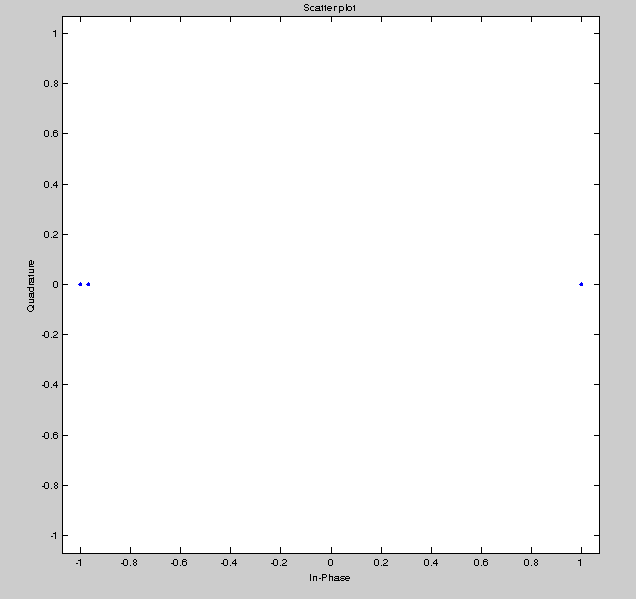
\includegraphics[width=150mm, scale = 0.9]{lab9/9_1}
   \caption{Сигнальное созвездие BPSK-модуляции}
\end{figure}

\begin{figure}[H]
   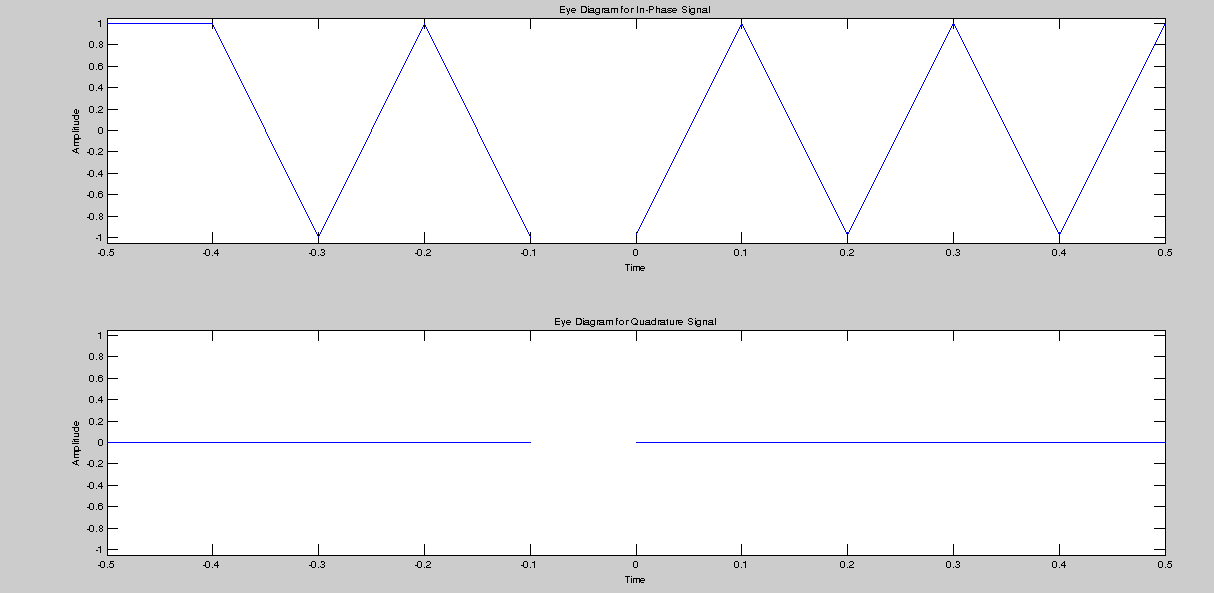
\includegraphics[width=150mm, scale = 0.9]{lab9/9_2}
   \caption{Глазковая диаграмма BPSK-модуляции}
\end{figure}




\begin{figure}[H]
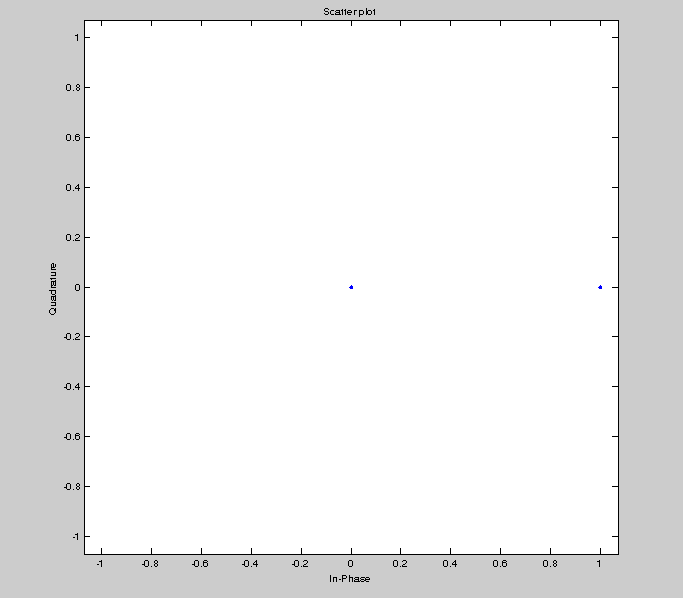
\includegraphics[width=150mm, scale = 0.9]{lab9/9_3}
   \caption{Сигнальное созвездие BPSK-демодуляции}
\end{figure}



\begin{figure}[H]
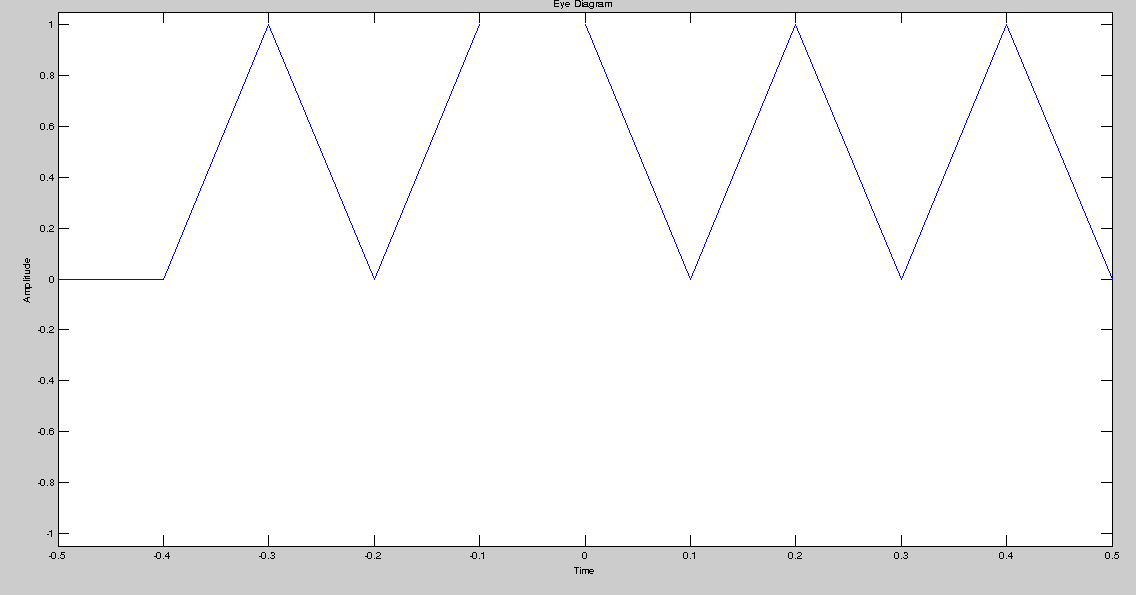
\includegraphics[width=150mm, scale = 0.9]{lab9/9_4}
   \caption{Глазковая диаграмма BPSK-демодуляции}
\end{figure}



\begin{figure}[H]
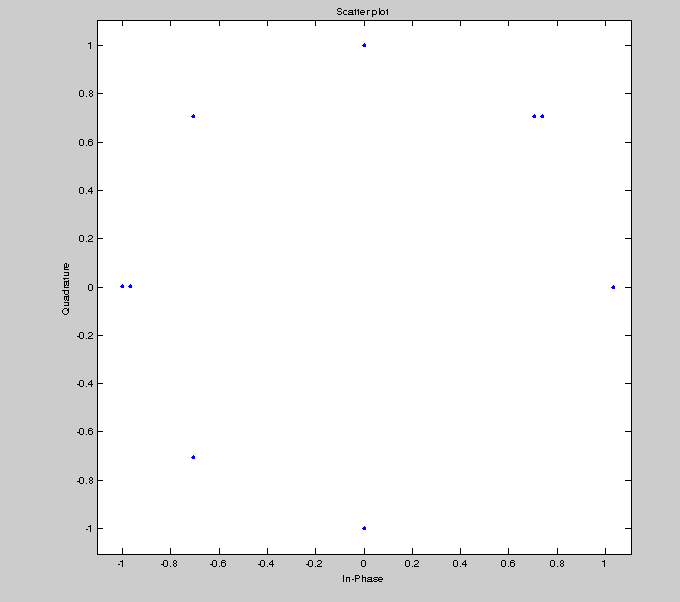
\includegraphics[width=150mm, scale = 0.9]{lab9/9_5}
   \caption{Сигнальное созвездие PSK-модуляции}
\end{figure}



\begin{figure}[H]
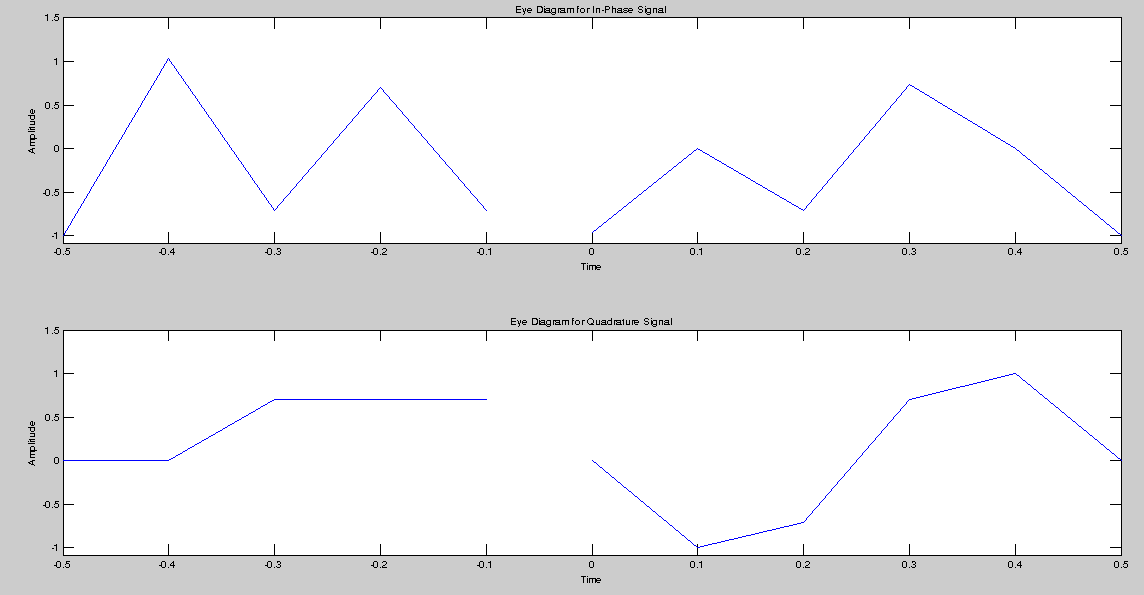
\includegraphics[width=150mm, scale = 0.9]{lab9/9_6}
   \caption{Глазковая диаграмма PSK-модуляции}
\end{figure}



\begin{figure}[H]
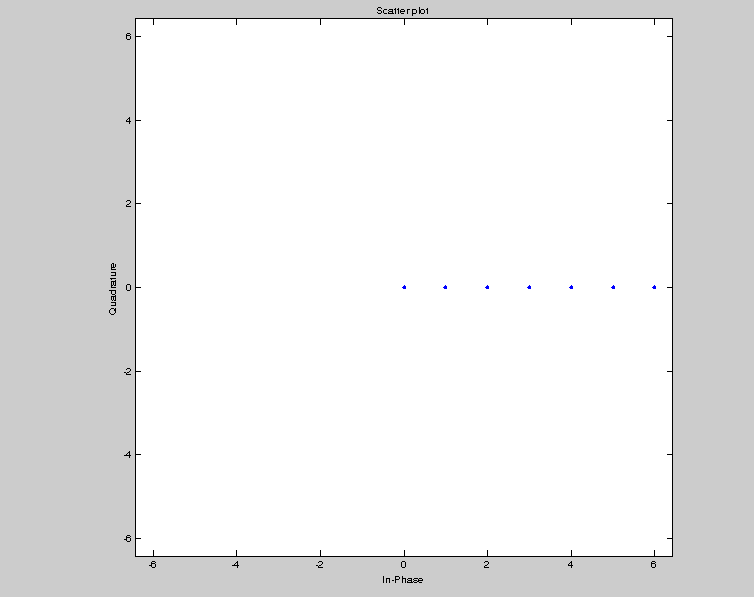
\includegraphics[width=150mm, scale = 0.9]{lab9/9_7}
   \caption{Сигнальное созвездие PSK-демодуляции}
\end{figure}



\begin{figure}[H]
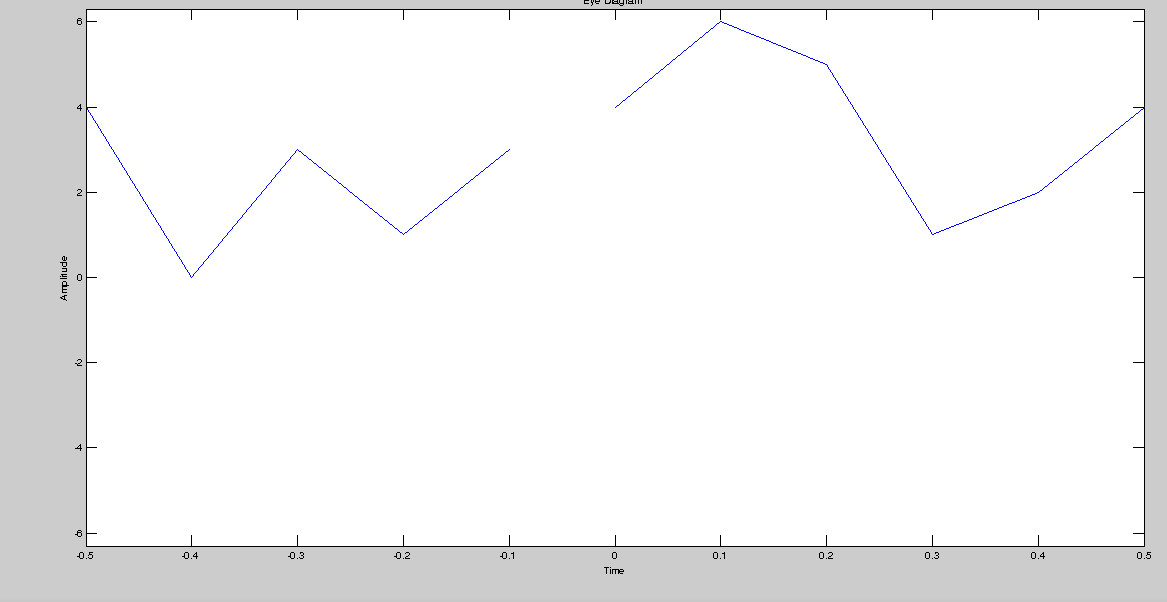
\includegraphics[width=150mm, scale = 0.9]{lab9/9_8}
   \caption{Глазковая диаграмма PSK-демодуляции}
\end{figure}



\begin{figure}[H]
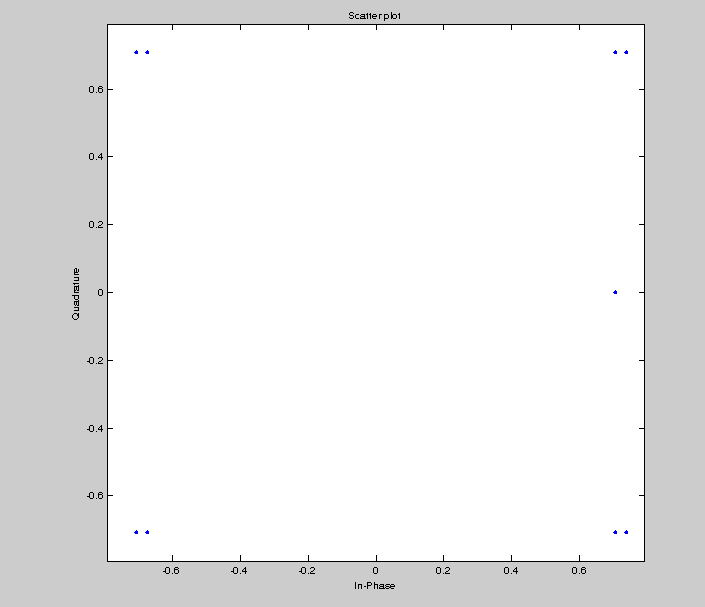
\includegraphics[width=150mm, scale = 0.9]{lab9/9_9}
   \caption{Сигнальное созвездие OQPSK-модуляции}
\end{figure}



\begin{figure}[H]
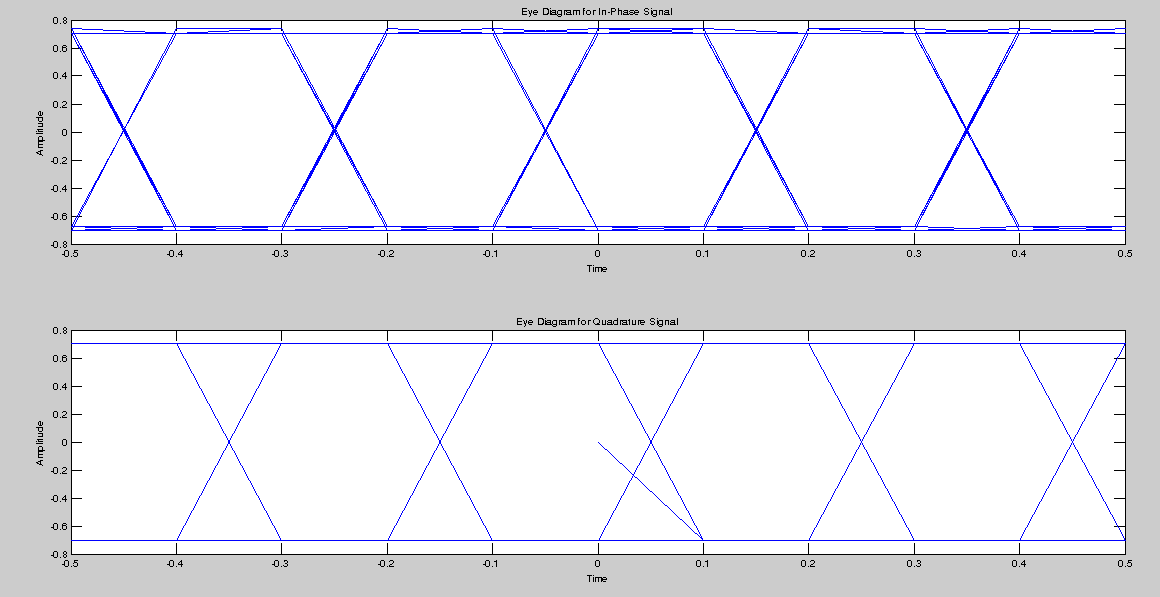
\includegraphics[width=150mm, scale = 0.9]{lab9/9_10}
   \caption{Глазковая диаграмма OQPSK-модуляции}
\end{figure}



\begin{figure}[H]
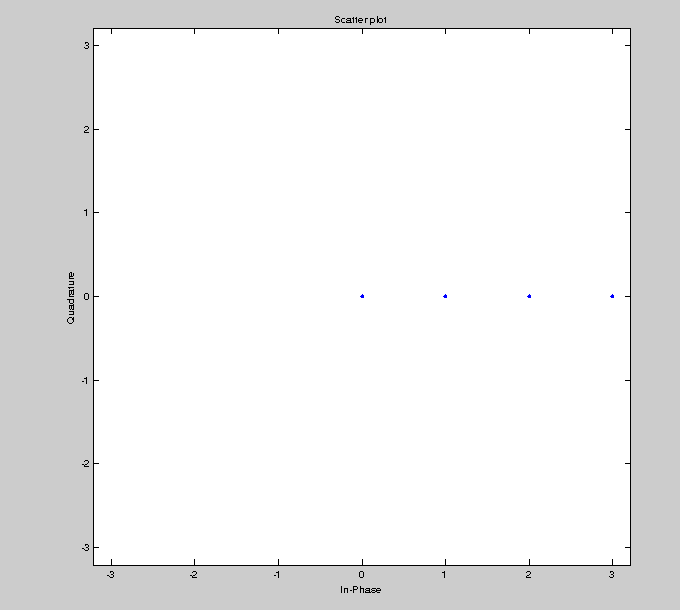
\includegraphics[width=150mm, scale = 0.9]{lab9/9_11}
   \caption{Сигнальное созвездие OQPSK-демодуляции}
\end{figure}



\begin{figure}[H]
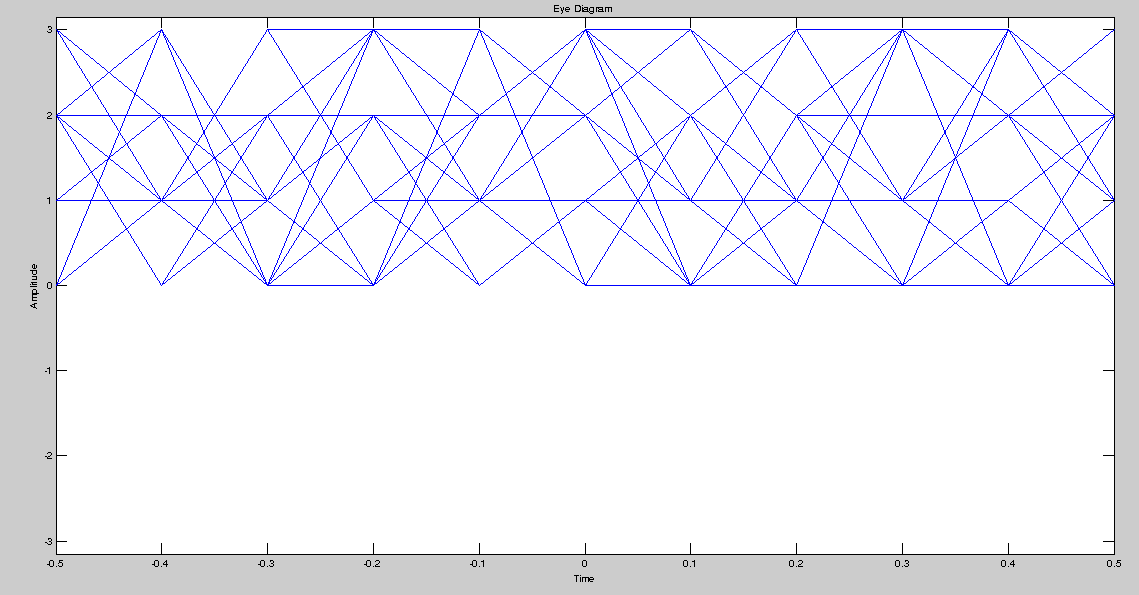
\includegraphics[width=150mm, scale = 0.9]{lab9/9_12}
   \caption{Глазковая диаграмма OQPSK-демодуляции}
\end{figure}



\begin{figure}[H]
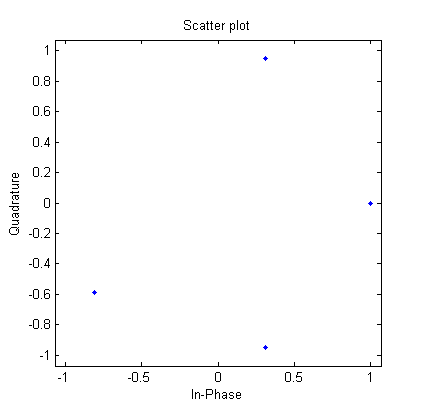
\includegraphics[width=150mm, scale = 0.9]{lab9/9_13}
   \caption{Сигнальное созвездие genQAM-модуляции}
\end{figure}



\begin{figure}[H]
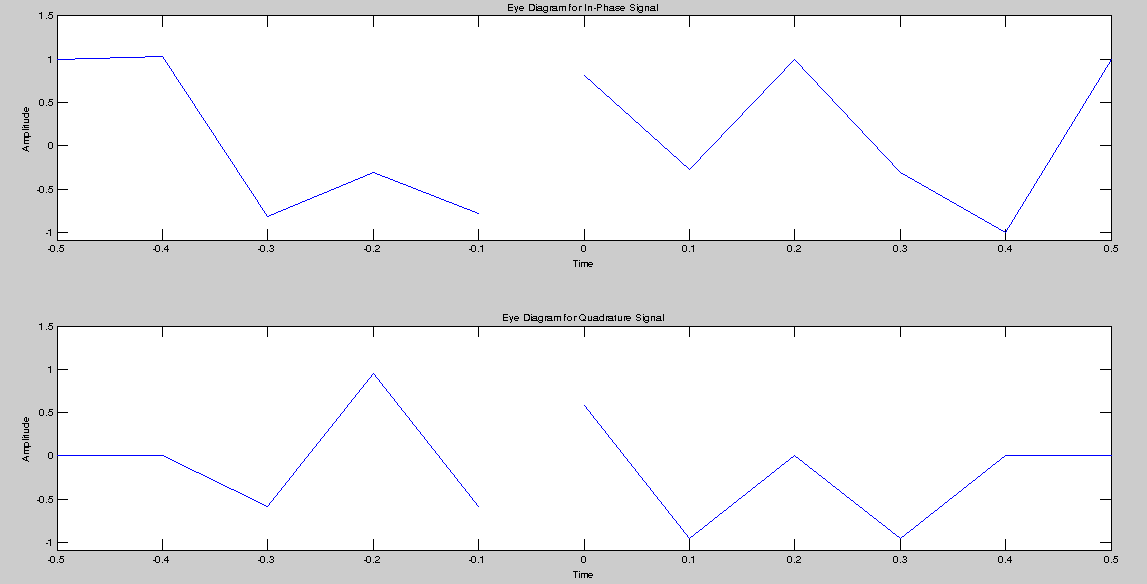
\includegraphics[width=150mm, scale = 0.9]{lab9/9_14}
   \caption{Глазковая диаграмма genQAM-модуляции}
\end{figure}



\begin{figure}[H]
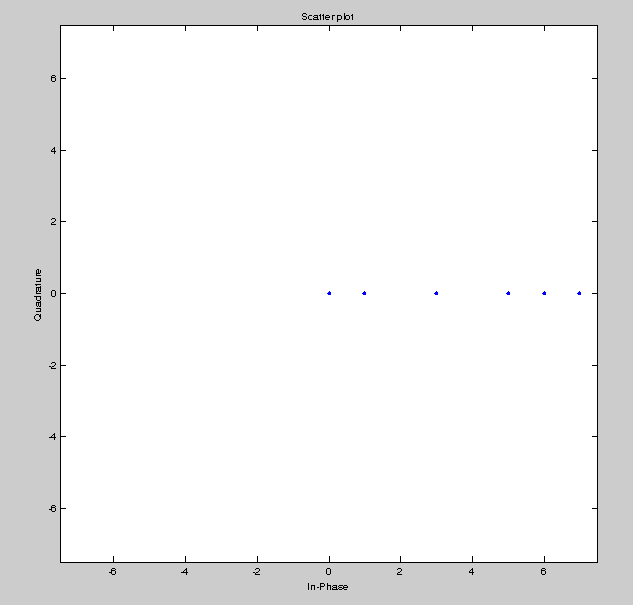
\includegraphics[width=150mm, scale = 0.9]{lab9/9_15}
   \caption{Сигнальное созвездие genQAM-демодуляции}
\end{figure}




\begin{figure}[H]
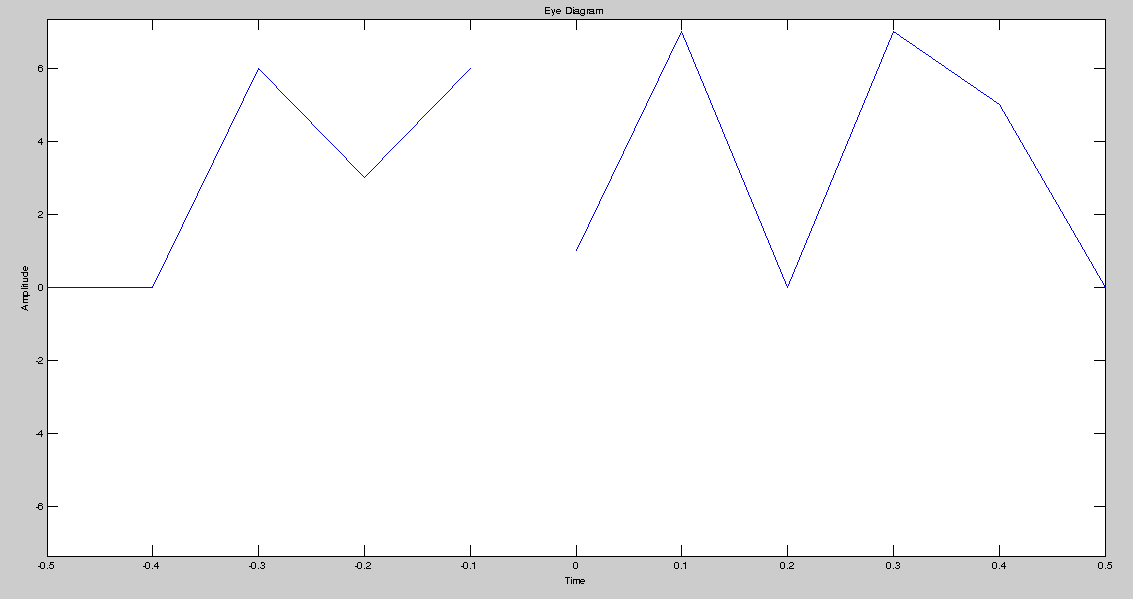
\includegraphics[width=150mm, scale = 0.9]{lab9/9_16}
   \caption{Глазковая диаграмма genQAM-демодуляции}
\end{figure}



\begin{figure}[H]
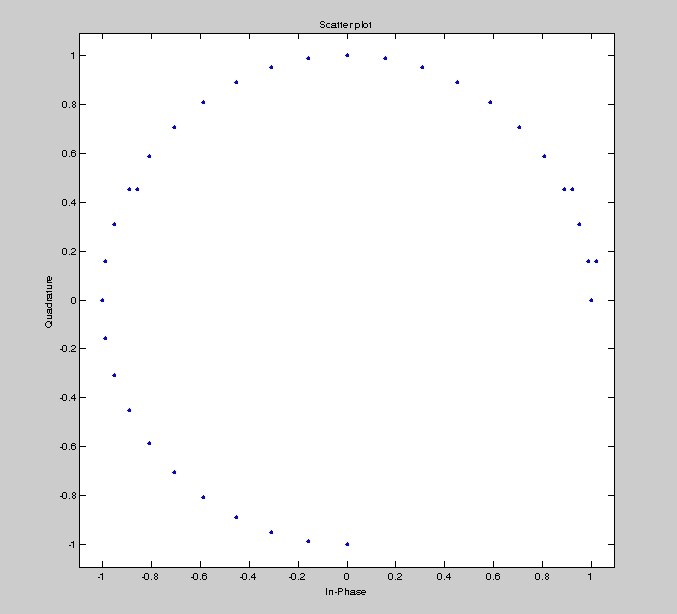
\includegraphics[width=150mm, scale = 0.9]{lab9/9_17}
   \caption{Сигнальное созвездие MSK-модуляции}
\end{figure}



\begin{figure}[H]
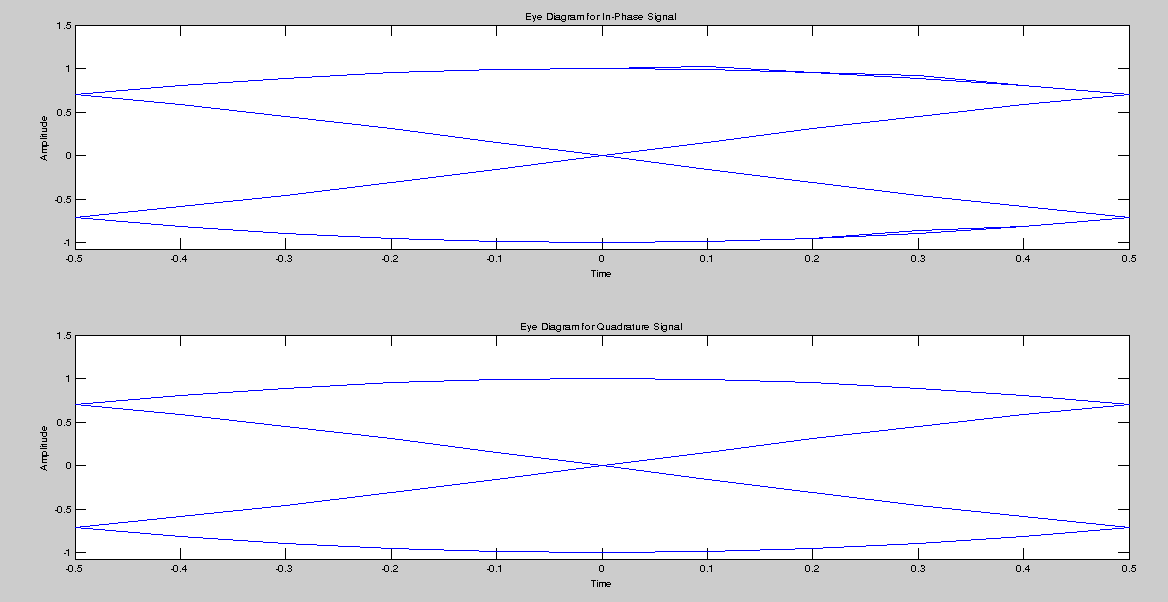
\includegraphics[width=150mm, scale = 0.9]{lab9/9_18}
   \caption{Глазковая диаграмма MSK-модуляции}
\end{figure}




\begin{figure}[H]
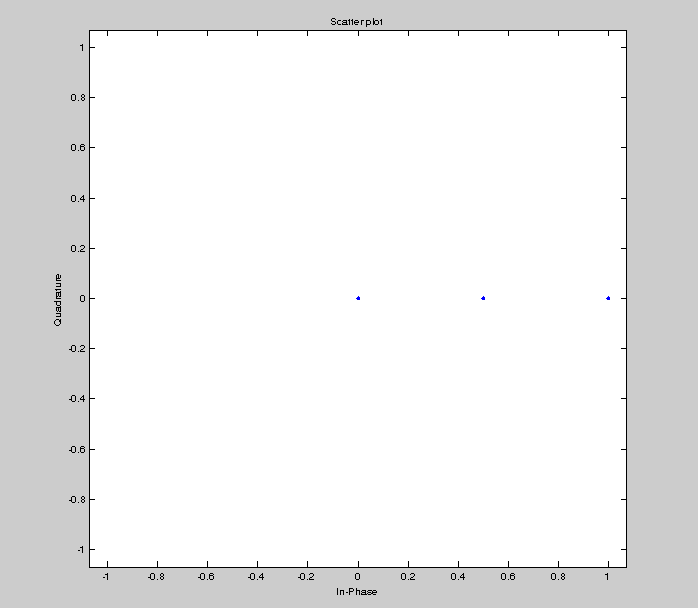
\includegraphics[width=150mm, scale = 0.9]{lab9/9_19}
   \caption{Сигнальное созвездие MSK-демодуляции}
\end{figure}



\begin{figure}[H]
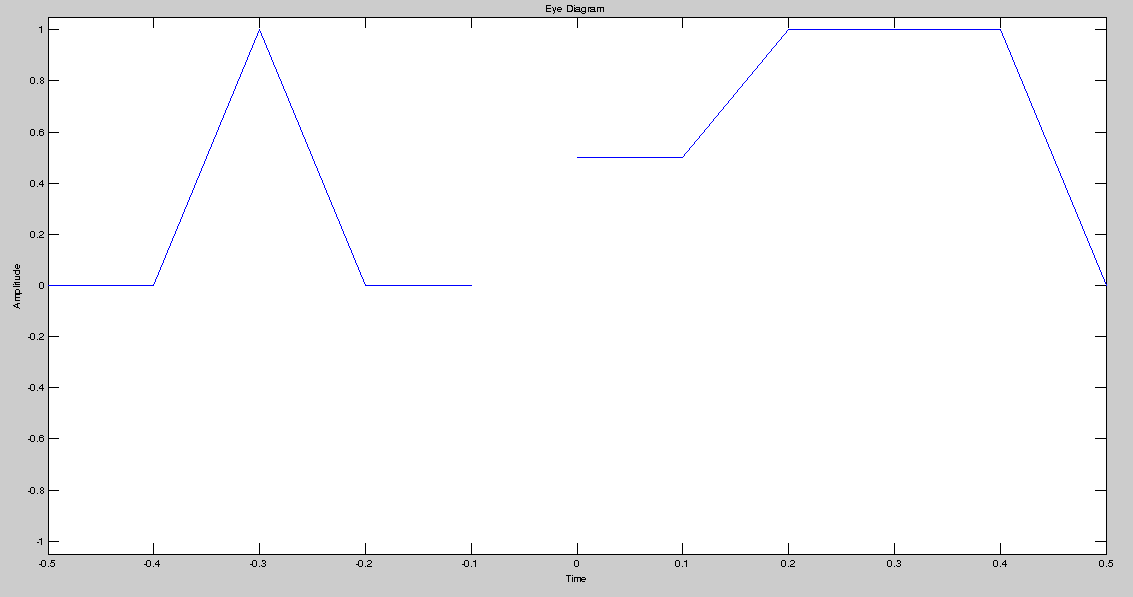
\includegraphics[width=150mm, scale = 0.9]{lab9/9_20}
   \caption{Глазковая диаграмма MSK-демодуляции}
\end{figure}



Смоделируем проделаные опыты при помощи simulink

\begin{figure}[H]
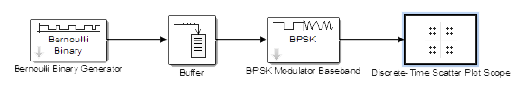
\includegraphics[width=150mm, scale = 0.9]{lab9/9_21}
   \caption{Модель BPSK-модуляции}
\end{figure}



\begin{figure}[H]
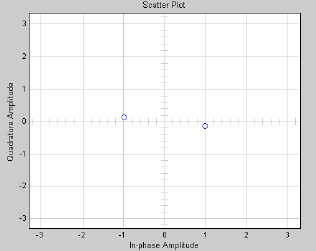
\includegraphics[width=150mm, scale = 0.9]{lab9/9_22}
   \caption{Сигнальное созвездие BPSK-модуляции}
\end{figure}



\begin{figure}[H]
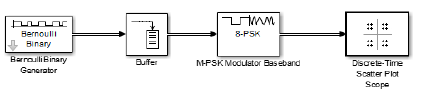
\includegraphics[width=150mm, scale = 0.9]{lab9/9_23}
   \caption{Модель PSK-модуляции}
\end{figure}



\begin{figure}[H]
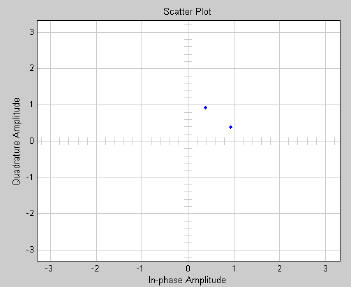
\includegraphics[width=150mm, scale = 0.9]{lab9/9_24}
   \caption{Сигнальное созвездие PSK-модуляции.}
\end{figure}



\begin{figure}[H]
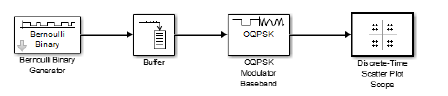
\includegraphics[width=150mm, scale = 0.9]{lab9/9_25}
   \caption{Модель OQPSK-модуляции}
\end{figure}



\begin{figure}[H]
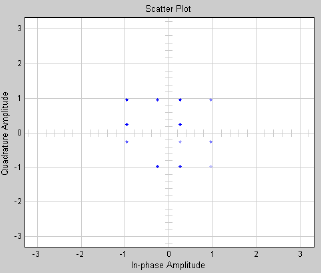
\includegraphics[width=150mm, scale = 0.9]{lab9/9_26}
   \caption{Сигнальное созвездие OQPSK-модуляции.}
\end{figure}



\begin{figure}[H]
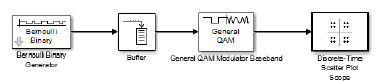
\includegraphics[width=150mm, scale = 0.9]{lab9/9_27}
   \caption{Модель genQAM-модуляции}
\end{figure}



\begin{figure}[H]
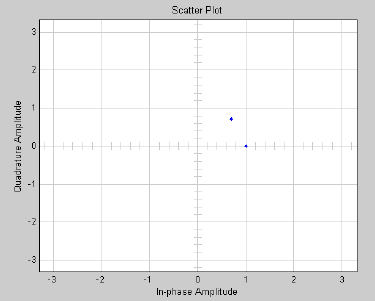
\includegraphics[width=150mm, scale = 0.9]{lab9/9_28}
   \caption{Сигнальное созвездие genQAM-модуляции}
\end{figure}



\begin{figure}[H]
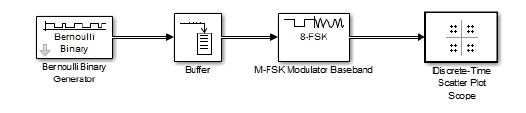
\includegraphics[width=150mm, scale = 0.9]{lab9/9_29}
   \caption{Модель MSK-модуляции}
\end{figure}



\begin{figure}[H]
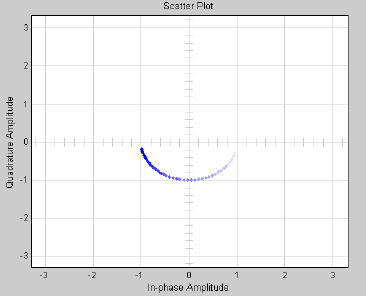
\includegraphics[width=150mm, scale = 0.9]{lab9/9_30}
   \caption{Сигнальное созвездие MSK-модуляции.}
\end{figure}


\section{Вывод}
Уровень модуляции определяет количество состояний несущей, используемых для передачи информации. Чем выше этот уровень, тем большими скоростными возможностями и меньшей помехоустойчивостью модуляция обладает. Число бит, передаваемых одним состоянием, определяется как $Log N$, где N — уровень модуляции. Таким образом, чем выше уровень модуляции, тем больше данных мы можем передать (или потерять) за единицу времени. Так же уровень модуляции напрямую зависит от приемника сигнала: чем более точный приемник, тем больший уровень модуляции мы можем задать.